\documentclass[11pt]{article}
\usepackage[letterpaper,margin=17mm,top=19mm,bottom=18mm,headheight=14pt,headsep=5mm,footskip=9mm]{geometry}
\usepackage[T1]{fontenc}
\usepackage{helvet}
\renewcommand{\familydefault}{\sfdefault}
\usepackage{amsmath,amssymb,array,booktabs,tabularx,fancyhdr,xcolor,tikz,enumitem,url}
\usetikzlibrary{arrows.meta}
\definecolor{ink}{RGB}{30,35,40}
\definecolor{redgood}{RGB}{185,63,68}
\definecolor{bluegood}{RGB}{41,107,164}
\color{ink}
\pagestyle{fancy}\fancyhf{}
\renewcommand{\headrulewidth}{0pt}\renewcommand{\footrulewidth}{0pt}
\fancyhead[L]{\small Week 58 / Fair division / Facilitator}
\fancyfoot[L]{\scriptsize Bellingham Math Circle / Week 58 / W58-guide-v1}
\fancyfoot[R]{\scriptsize\thepage}
\setlength{\parindent}{0pt}\setlength{\parskip}{2.2mm}
\setlist[itemize]{nosep,leftmargin=4.7mm,topsep=1mm}
\newcommand{\heading}[1]{\par\vspace{1.5mm}{\large\bfseries #1}\par\vspace{.8mm}}
\newcommand{\subhead}[1]{\par\vspace{1mm}\textbf{#1}\par}
\newcommand{\adult}[1]{\textbf{Adult prompt.} #1\par}
\newcommand{\page}[1]{\newpage\heading{#1}}
\renewcommand{\arraystretch}{1.25}
\newcolumntype{L}[1]{>{\raggedright\arraybackslash}p{#1}}
\begin{document}
\heading{Mathematical overview}
For a \textbf{complete allocation with fixed, nonnegative additive values}, envy-freeness implies proportionality. For \textbf{two people}, the two conditions are equivalent. For \textbf{three people}, proportionality can hold while every person envies someone else. Whole items can make both conditions impossible. With a divisible, nonatomic resource, two-person cut-and-choose can always give an envy-free, proportional allocation.

\subhead{The model and the comparisons}
Every item or piece goes to exactly one recipient; nothing is hidden or discarded. A person values a bundle by adding that person's values for its contents. Different people can have different values, and zero is permitted. Keep the same observer's preference card for every tray in one comparison. A tie passes. A referee is not an extra recipient.

For observer $i$, let $T_i$ be the value of everything, and let $s_i$ be the value of the observer's own bundle. With $n$ recipients, \emph{proportional} means $s_i\ge T_i/n$ for every person. \emph{Envy-free} means $s_i$ is at least that observer's value of each other person's bundle. Comparing A's own score with B's own score answers neither question. Equal counts and equal lengths need not mean equal value.

\subhead{Why the relationships hold}
If every one of the $n$ bundles is worth at most $s_i$ to observer $i$, adding their values gives $T_i\le n s_i$. This proves envy-free $\Rightarrow$ proportional. With two people the other bundle has value $T_i-s_i$; hence $s_i\ge T_i/2$ exactly when $s_i\ge T_i-s_i$. With three people, being above one third of the total need not make the own bundle largest. Problem 6 supplies a complete example with own value 4, competing values 8 and 0, and total 12.

\subhead{The divisible-resource theorem and its limits}
The cutter makes two pieces of exactly equal \emph{own} value. The chooser takes a piece of maximum \emph{own} value, and the cutter receives the remainder. The cutter is indifferent and has half the cutter's total. The chooser gets at least half the chooser's total and does not envy the remainder. Thus both conditions hold.

Existence of an exact equal-value cut needs divisibility and nonatomic values: value cannot be trapped in an indivisible positive-value point or card. For an interval, continuity of accumulated value from the left suffices. The packet's two constant-density color panels have this property. A scissors cut only approximates the exact theorem. Cutting at the color join is not necessarily equal-value. Negative chores, changing tastes, complementary values and payments are outside this activity's model. Simple cut-three-and-let-two-choose does not inherit the two-person guarantee.

\subhead{What children are meant to discover}
Pages 1--3 and 5 (approximately Grades 2--5) offer moving, choosing and cutting: two trays can suit different tastes, and allowing a split can remove an obstruction. Pages 4, 6 and 7 (approximately Grades 3--5, by readiness) connect those trials to a guarantee, a counterexample and a general argument. K--1 has an optional oral entry, not a printed packet. Experiments suggest patterns; a full small catalog or an explanation establishes the claimed result. No child must finish all seven pages in one visit.

\page{Running the hour with three anchored adults}
\subhead{Shared launch: about 5 minutes after movement}
Allow about five minutes of running or movement first. At the tables, let children handle the cards and trays for a minute before assigning a problem. Bring everyone briefly together. Use the page-1 non-task picture: three neutral counters become two trays; the chooser takes a tray first and the divider takes the remainder. Say: ``Put everything into two trays. Your partner chooses first. You get the other tray. Then we check whether either person wants to trade.'' Let two children make that demonstration. It teaches the turn convention without giving the target allocations.

Next put one red card in one tray and one blue card in the other. Use A's preference-card dots to value both trays. Slide that same preference card from one tray to the other; do not switch observers midway. Then use B's card for both trays to show different scores. Keep it brief. At the strip table later, use page 3's 150 mm panel worth 2 $\to$ two 75 mm lengths $\to$ value 1 each before a first cut. The numerical card means a whole panel's value, not every fragment's value.

\subhead{The fixed tables: 35--40 minutes of work}
\textbf{KK11: parent volunteer, two pairs.} Use the page-1 card subset and two trays per pair, with oral directions. Children decide the division and the first choice; the adult reads preferences and can count dots with them. Repeat role swaps and ask each to point to the tray they would rather keep. About 15--25 minutes of this may be ample. If fixed numerical preferences are not retained, use children's own stated tastes for an oral divide/choose investigation; describe it as preference play, without a numerical fairness claim. For a ready pair, Problem 5's three identical-value reds is a concrete continuation. The adult can cut the replacement square where children mark it. Do not give a K--1 catalog or universal-proof assignment.

\textbf{3333: second mathematician, two pairs.} Begin Problem 1 for 10--15 minutes. Choose Problem 2's pooled catalog or Problem 5's whole/split contrast for the next 15--20 minutes. A pair ready for length-based value can instead spend that time on Problem 3, including both cutting roles. A sensible first stopping point is one checked successful allocation plus one changed-resource trial; the complete catalog and proof can wait.

\textbf{445: organizer, one pair and a rotating referee.} Start with 5--10 minutes of Problem 1 or 2. Continue with Problem 3 and, when ready, Problem 4 for 15--20 minutes. Reserve the last 10 minutes for Problem 6 \emph{or} 7, or save both for a return. The referee keeps the observer fixed, checks that every piece is allocated, and rotates after each trial. Problem 6 instead has three actual recipients and three trays.

Allow a brief stretch or stand-and-reset break when attention fades. End with 5--7 minutes of sharing a saved allocation, a cut or an impossibility argument. Keep adults anchored; do not rely on the organizer circulating to operate every trial. The single adult at each four-child table supports two pairs in turn, so start only one unfamiliar cutting procedure at a time.

\subhead{Readiness gates, not age guarantees}
Adult reading and recording are acceptable; children must retain the division and choice decisions. Pages 1--2 need small sums (to 10), labels and one fixed observer. Page 3 additionally needs measuring and value proportional to length within one color. Page 5 needs whole counts to 3 and equal-area halves. Pages 6--7 need sums to 12, one third of 12, comparisons of three trays and the difference between an example and ``always.'' Exact thirds in strip scores are an optional extension. If an adult must make the mathematical choices, return to a concrete earlier route.

\page{Print and assemble the actual kit}
Prepare \textbf{five pair kits}: two for KK11, two for 3333, one for 445; also one separate three-person upper kit. Print materials single-sided on US Letter at \textbf{100\%, actual size}; pages 2--5 are landscape. The following counts use the delivered ten-page materials PDF.

\begin{tabularx}{\linewidth}{@{}L{20mm}L{22mm}X@{}}\toprule
Pages & Copies each & Result for the whole group\\\midrule
1 & 5 & 25 reusable 25 mm squares: R1,R2,R3,B1,B2 per pair; plus 5 separate cuttable paper R3 replacements.\\
2 & 5 & 10 A/B preference cards, each 100 $\times$ 150 mm.\\
3 & 5 & 10 U/V preference cards, each 100 $\times$ 150 mm.\\
4 and 5 & 1 & 3 upper observer cards, each 100 $\times$ 150 mm; 3 whole X/Y/Z panels, each 50 $\times$ 40 mm.\\
6--10 & 5 & 100 strip halves, each 150 $\times$ 40 mm: 50 finished 300 $\times$ 40 mm strips, 10 per pair.\\\bottomrule
\end{tabularx}

\textbf{Full stock: 42 material sheets}, with ten strips per pair for retries and returns. \textbf{Smaller first-route stock: 27 sheets}: five copies each of pages 1,2,3,6,7 and one each of pages 4,5. Eight halves/four strips per pair (20 strips total) cover both Problem 3 roles, the Problem 4 join-cut and one retry. More trials need more strip copies. Card and upper-kit counts are unchanged; prepare only the named goods above, with no green goods.

Suggested first-route student supply: two copies each of pages 1,5 for KK11; two each of pages 1,2,3,5 for 3333; one of all seven for 445: \textbf{19 student sheets}. Share one record per pair; adults retain unused pages. Adjust this subset to the chosen route.

\subhead{Assembly and resets}
Mount \emph{only} R1,R2,R3,B1,B2 from material page 1 on sturdy backing; cut their outside borders. Leave the separate paper R3 unmounted. Cut out preference cards and upper panels. Supply ten 150--180 mm whole-card trays (two per pair), three upper trays, five rulers, pencils, blank paper, tape and three adult-held scissors. Three neutral counters or blank paper disks serve the launch only.

For strips, use two labelled flat paper/table zones per pair, each at least 220 $\times$ 100 mm, with clear space for the initial 300 $\times$ 40 mm strip, or larger trays. Paper-marked table zones suffice; no purchase is needed.

Cut strip halves on outside borders. Match numbers and butt-join red left, blue right, 150+150=300 mm, with no gap or overlap; tape only on the back. Separate pair kits where numbers repeat. A cut parallel to the join crosses the 40 mm width; measure from the red/left end. Student sketches are schematic; cut the separate full-size materials.

For Problem 1 set out R1,R2,R3,B1 with A/B; for Problem 2 use R1,R2,B1,B2 with A/B; for Problem 5 use R1,R2,R3 with U/V. Put every unused good away. In Problem 5's second trial, \textbf{remove sturdy R3 before adding paper R3}; the total stays three cards' value. The red icon identifies the square; value follows the area of the entire square, not the inked circle. Only explicitly splittable resources may be cut. Problem 6 uses its separate observer cards, not the A/B color cards.

\subhead{Physical pretests still to perform}
\textbf{Unperformed physical checks}: print scale/orientation, 300 mm seam flatness, card/tray/work-zone footprint, replacement-half handling, scissors timing, kit resets and the parent volunteer's fixed-observer rehearsal. Staffing, route timing, child independence and classroom piloting are untested. Check 100 mm bars with a ruler; rehearse one divide/choose/reset and both strip roles with the actual adults and materials.

\page{Problems 1 and 2: whole-card allocations}
\subhead{Problem 1 (student page 1): three reds and one blue}
With A's values $(R,B)=(3,1)$ and B's $(1,3)$, totals are 10 and 6. Both keep their own tray exactly when A gets value at least 5 and B at least 3. There are \textbf{four successful labeled complete allocations}:

\begin{tabularx}{\linewidth}{@{}L{31mm}L{33mm}X@{}}\toprule
A receives & B receives & Own / other values: A; B\\\midrule
R1,R2 & R3,B1 & $6/4$; $4/2$\\
R1,R3 & R2,B1 & $6/4$; $4/2$\\
R2,R3 & R1,B1 & $6/4$; $4/2$\\
R1,R2,R3 & B1 & $9/1$; $3/3$\\\bottomrule
\end{tabularx}

For completeness, let A get $r$ reds and $b$ blues. A needs $3r+b\ge5$. B's own value is $6-r-3b$, so B needs $r+3b\le3$. If $b=1$, these inequalities cannot both hold. If $b=0$, $r=2$ or 3. The three choices of two labeled reds and the one choice of all three exhaust the possibilities, out of $2^4=16$ allocations.

The two-red / red-plus-blue partition succeeds whichever person divides: B strictly chooses red-plus-blue, and A strictly chooses two reds. In the all-red / blue partition, if B divides, A strictly chooses all reds and the result succeeds. If A divides, B sees a $3$--$3$ tie: choosing blue succeeds, but choosing all reds leaves A with blue and fails A's check. \textbf{Ties are allowed; they do not force a particular choice.} Finding a successful allocation is not a whole-card guarantee for arbitrary divider decisions.

\adult{``Keep A's card here. What does A think of each tray? Now use B's card for both.'' If needed, move dot counters beside each tray. Save labels in one printed record. A useful failed trial gives A one red and the blue: A sees 4 versus 6, although the trays have equal counts.}

Allow 10--15 minutes or longer; repeats with roles swapped are substantive work. Do not require the four-case proof before continuing.

\subhead{Problem 2 (student page 2): two reds and two blues}
Each observer's total is 8 and half is 4. Exactly \textbf{five} of the 16 labeled complete allocations are envy-free; all five, and only those five, are proportional for both people:

\begin{tabularx}{\linewidth}{@{}L{31mm}L{33mm}X@{}}\toprule
A receives & B receives & Own / other values: A; B\\\midrule
R1,R2 & B1,B2 & $6/2$; $6/2$\\
R1,B1 & R2,B2 & $4/4$; $4/4$\\
R1,B2 & R2,B1 & $4/4$; $4/4$\\
R2,B1 & R1,B2 & $4/4$; $4/4$\\
R2,B2 & R1,B1 & $4/4$; $4/4$\\\bottomrule
\end{tabularx}

A's red count $r$ and blue count $b$ must satisfy $3r+b\ge4$ and $r+3b\le4$. The only count pairs are $(2,0)$ and $(1,1)$: one color split plus $2\cdot2=4$ mixed splits. Reversing the preferred color split fails both checks, whereas exchanging labels within mixed splits creates distinct valid records. The sixth recording box is spare space, not evidence for a sixth solution.

Fill the saved-record table for \emph{one unchanged allocation}: the color split gives rows $(6,2,8,4)$ for both; a mixed split gives $(4,4,8,4)$ for both. Let pairs pool catalogs over 15--25 minutes. A completeness hint is to sort by A's red/blue counts.

\page{Problems 3 and 4: cutting, choice and guarantee}
\subhead{Problem 3 (student page 3): the exact physical model}
Every strip is 300 mm long, red on $[0,150]$ and blue on $[150,300]$. A whole red/blue panel is worth $(3,1)$ to A and $(1,3)$ to B. Partial-panel value follows length within that color. Each observer's total is 4, so the cutter seeks own value 2 on each side.

\begin{center}
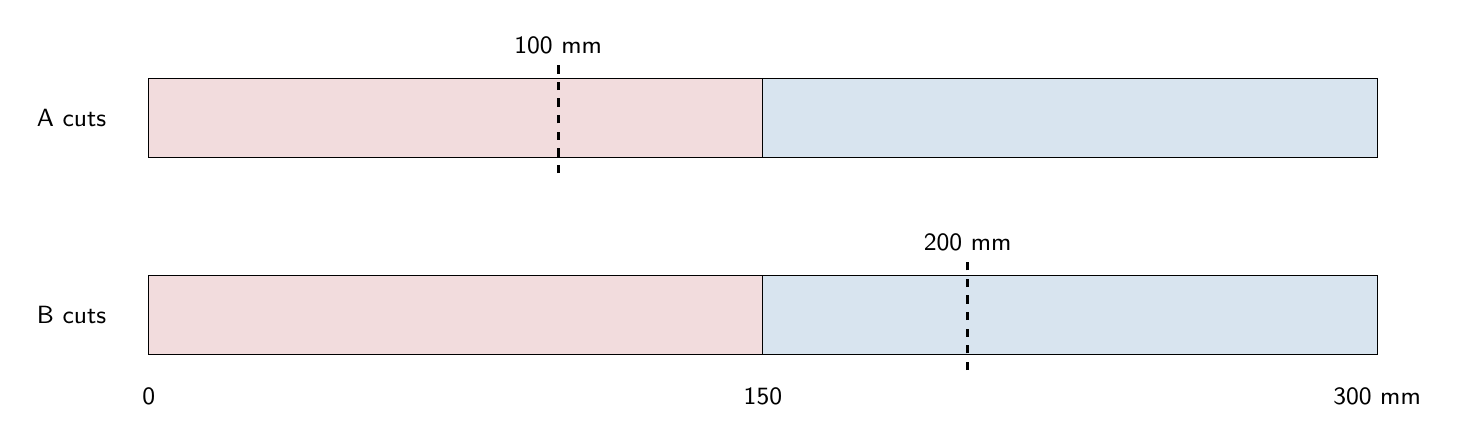
\begin{tikzpicture}[x=.52mm,y=1mm]
\foreach \y/\c/\cut/\who in {25/A/100/B,0/B/200/A}{
 \draw[fill=redgood!18] (0,\y) rectangle (150,\y+10);
 \draw[fill=bluegood!18] (150,\y) rectangle (300,\y+10);
 \draw (150,\y)--(150,\y+10);
 \draw[dashed,line width=1pt] (\cut,\y-2)--(\cut,\y+12);
 \node[anchor=east,font=\small] at (-8,\y+5){\c\ cuts};
 \node[font=\small,anchor=south] at (\cut,\y+12){\cut\ mm};
}
\node[font=\small,anchor=north] at (0,-3){0};
\node[font=\small,anchor=north] at (150,-3){150};
\node[font=\small,anchor=north] at (300,-3){300 mm};
\end{tikzpicture}
\end{center}

\begin{tabularx}{\linewidth}{@{}L{29mm}L{28mm}L{33mm}X@{}}\toprule
Cutter / distance & A: left, right & B: left, right & Chooser and final assignment\\\midrule
A / 100 mm & $2,2$ & $\frac23,\frac{10}3$ & B takes right; A takes left.\\
B / 200 mm & $\frac{10}3,\frac23$ & $2,2$ & A takes left; B takes right.\\\bottomrule
\end{tabularx}

For A, $3(100/150)=2$; the rest is $3(50/150)+1=2$. B values A's left piece at $100/150=2/3$ and the right at $50/150+3=10/3$. For B, the left piece has value $1+3(50/150)=2$, so the cut is at 200 mm; A's values are $3+50/150=10/3$ and $100/150=2/3$. These exact cuts are unique because both panel densities are positive. Both roles finish with A on the left and B on the right, but the boundary and their values differ. Preserve each role's marked sketch and distance as its recoverable record.

Children may locate equal value by trying lengths or dividing a panel into equal parts; do not dictate the 100/200 mm marks at the outset. Give 15--25 minutes for both roles, fresh strips and retries. Adults cut at the child's mark. Exact fractional scores are a fraction-ready return question, not a required page-3 computation. \adult{``This card values the whole panel. What would half of this color be worth? Which observer are we checking now?''}

\subhead{Problem 4 (student page 4): both answers are yes}
For an exact equal-own-value cut, the cutter receives half of the cutter's total and values both pieces equally. The chooser receives a weak maximum of two pieces: the larger is at least their average, half of the chooser's total. The chooser also values that piece at least as much as the remainder. Thus each receives a proportional share and neither envies. This proves the guarantee for any preferences satisfying the stated model, rather than only the two experimental cuts.

\textbf{Join-cut countertrial: it fails both all-person checks.} Both people now use A's preferences; the red half is worth 3 and the blue half 1 to each. At the 150 mm join cut, the chooser takes red (3) and the cutter gets blue (1). Total is 4, half is 2: the cutter is below half and envies red. The chooser passes both checks. The cutter has failed the equal-own-value assumption, so this does not refute the theorem. Equal lengths are insufficient. Allow 5--15 minutes, or return after more cuts. Never call a measured scissors trial an exact proof; preserve the child's argument even if an adult writes it.

\page{Problem 5: an obstruction removed by a split}
\subhead{Student page 5: U and V value each red at 1}
First set out exactly R1,R2,R3 and the U/V cards. Cards stay whole. Every complete allocation has one of the count pairs $(0,3),(1,2),(2,1),(3,0)$. The smaller tray is strictly less valuable to its owner. Therefore \textbf{no envy-free whole-card allocation exists}. Both must have at least half of total value 3 to be proportional, which is impossible with whole-card integer values. Among the $2^3=8$ labeled allocations, 1 has U's count 0, 3 have count 1, 3 have count 2 and 1 has count 3; none passes either all-person condition.

\adult{``Leave all three cards in the two trays. Which person would rather trade? Can either tray have one and a half whole cards?'' Let children move the objects and exhaust count pairs. A paired-and-leftover drawing is a valid impossibility explanation. Do not settle for ``we tried a few and failed'' if the child is ready to explain all cases.}

\subhead{Second trial: replace, then cut}
Put sturdy R3 away. Introduce the \emph{single} unmounted paper R3 in its place; keep only sturdy R1,R2 and paper R3. Do not add a fourth red item. The paper square's entire area has value 1 to both U and V, with uniform value by area. The red circle is only its identifying icon. A half-square has value $1/2$, whether or not that half contains half the printed icon.

Give each person one whole card and one equal-area half of paper R3. Both now see own value $1+1/2=3/2$ and other value $3/2$. They are tied, envy-free and proportional. R1 and R2 can be exchanged. A cut down the middle of the square or along its diagonal gives equal areas. Other cuts are permissible if the two recipients' total paper areas are equal; the paper can be split into more pieces.

This characterizes every successful allocation under the second trial's rules: one whole card must go to each person, because putting both whole cards in one tray gives it value at least 2, while the other tray can have value at most 1. Then each must receive exactly half of the paper's area. For a \emph{fixed} pair of labeled half-squares H1,H2 there are four labeled successful assignments: either whole card with either half for U, and the complementary pair for V. This finite count does not enumerate all possible cutting shapes.

\subhead{Facilitation and stopping point}
Give the whole-card trial 5--10 minutes and the replacement trial another 5--10, extending if children are engaged. The mathematical change is divisibility, not a different meaning of envy. Compare the intact three-card trial with the saved split allocation side by side on paper. A child can make the explanation without writing fractions: ``Each gets one card and an equal piece of the last card.''

If tiny halves are awkward, the adult should handle the cut at the child's marked line and help move the pieces. Equal-area half-square handling has not been rehearsed. Do not quietly enlarge just the replacement, introduce the sturdy R3 alongside it, discard a leftover, or switch to personal tastes during this fixed U/V trial. Those alter the stated resource or preferences.

\subhead{A return question with a new mathematical job}
After the obstruction is clear, ask whether splitting \emph{one} card is enough for any odd number of identical positive-value cards shared by two people. Pair the whole cards between trays and split the final one equally. Even totals need no split. Conversely, an odd number of whole identical positive-value cards cannot be divided equally. This is an object-based parity argument, not another numerical catalog. Let children choose a small odd total with extra home-made identical cards on a later visit; record those as added materials, not contents of this five-card kit.

\page{Problems 6 and 7: three people and general claims}
\subhead{Problem 6 (student page 6): preserve the initial state}
Use three trays and the separate panel cards. Initially A has X, B has Y, C has Z. Fill the printed table for \emph{this unchanged allocation}, using one observer row at a time:

\begin{center}
\begin{tabular}{@{}lrrrr@{}}\toprule
Observer & A's tray (X) & B's tray (Y) & C's tray (Z) & One third of all\\\midrule
A & 4 & 8 & 0 & 4\\
B & 0 & 4 & 8 & 4\\
C & 8 & 0 & 4 & 4\\\bottomrule
\end{tabular}
\end{center}

Each total is 12 and each own tray is worth 4. The initial division is \textbf{proportional for all three, envy-free for none}: A envies B's Y, B envies C's Z, C envies A's X. Compare rows, not the three diagonal scores. A value of zero does not remove a panel or an observer from the problem.

After saving that table, physically rearrange to \textbf{A:Y, B:Z, C:X}. Each person receives their favorite whole panel worth 8 and values the other two at 4 and 0. This is envy-free and proportional. Do not update the original table one move at a time. Save the repaired allocation on the page's lines or blank paper, with a new state label.

Among the six ways to give one panel each, only the repaired assignment is envy-free. Exactly two are proportional: initial $A:X/B:Y/C:Z$ and repaired $A:Y/B:Z/C:X$. This exhausts all $3^3=27$ complete whole-panel allocations, including empty trays: proportionality requires positive own value, so each needs a panel; three panels force one each. Envy-freeness then forces each unique favorite.

Allow 10--20 minutes, rotating observer or recipient roles. Hint: ``For A, compare all three trays using A's row.'' After the static check ask which panel each wants. One person's envy suffices; no mutual exchange preference is required. This is not a claim that three-person envy-free cake division is impossible.

\subhead{Problem 7 (student page 7): all four answers}
\begin{tabularx}{\linewidth}{@{}L{24mm}L{53mm}X@{}}\toprule
Recipients & Proportional but not envy-free? & Envy-free but not proportional?\\\midrule
Two & No. The two conditions coincide. & No. The two conditions coincide.\\
Three & Yes. Problem 6's initial allocation. & No. Envy-free implies proportional.\\\bottomrule
\end{tabularx}

For \textbf{two people}, fix one observer. Write $s$ for own value and $t$ for the other tray's value. Total is $s+t$. Then
\[
 s\ge\frac{s+t}{2}\quad\Longleftrightarrow\quad 2s\ge s+t
 \quad\Longleftrightarrow\quad s\ge t.
\]
Repeat for the other observer. The printed boxes use one observer's values at a time.

For \textbf{three people}, Problem 6's initial rows $(4,8,0)$, $(0,4,8)$ and $(8,0,4)$ supply the yes example. For the no answer, fix an observer whose own value $s$ is at least each other value $t,u$. Then $s+t+u\le3s$, so $s\ge(s+t+u)/3$. Repeat for all observers. Three equal-or-smaller drawn bars can express this proof; algebra is optional. An all-zero observer passes both tests and still counts. Allow 10--20 minutes after concrete examples, possibly on another visit. Invite one observer's comparison before offering algebra.

\page{Return visits, extensions and what to record}
\subhead{A theme can support several meetings}
The first hour need not reach the definitions, exact catalog, cutting proof and three-person example all at once. Keep familiar trays and preference cards available on a return. Open with a child's saved record and a short replay of the action. Choose a new mathematical question, rather than repeating the same scores because a page remains unfinished.

\textbf{Visit A: divisions with differing tastes.} Problems 1 and 2 can occupy a whole main-table hour. Start with attempts, pool a collection of successes, then ask how to know no cases are missing. The two-red / red-plus-blue partition from Problem 1 leads to a separate question about which divider/chooser roles make success certain and why a tie matters. Let the youngest table remain with choosing and keeping trays.

\textbf{Visit B: when splitting changes possibility.} Return through Problem 5 and then Problem 3. One splits an otherwise indivisible square; the other values a continuous strip by color density. Ask why equal counts, equal area and equal length are different from equal \emph{own} value. Children who are ready can compare the unsplit obstruction with the cut-and-choose guarantee; keep the younger oral route concrete.

\textbf{Visit C: guarantee and its assumptions.} Use Problem 4 after several physical cuts, then Problem 7's two-person argument. Try a deliberately unequal-value cut and identify whose guarantee survives: a chooser who selects a weak maximum still receives at least half and does not envy, but the cutter may fail. Use the join-cut countertrial instead of introducing another preference system. Exact strip scores with thirds deepen the same saved cuts for fraction-ready children.

\textbf{Visit D: three recipients.} Revisit the fixed initial Problem 6 allocation, then repair it and connect it to Problem 7. The distinction between a checked counterexample and a universal implication is the new direction. Do not rush into a full three-person trimming algorithm. Procaccia's Selfridge--Conway background uses trimming and a separate allocation of trimmings; it would require a distinct later plan and prepared materials.

\subhead{Optional deeper questions, with their destinations}
\textbf{Cutting error.} For a cutter's mark within the same color as the ideal cut, an error of $e$ mm changes the cutter's piece values from $(2,2)$ to $(2+e/50,2-e/50)$, with the signs reversed when considering the complementary side. Thus the smaller cutter piece is $2-|e|/50$. This uses the relevant density $3/150=1/50$ per mm. It quantifies an approximation; it does not turn it into exact envy-freeness. The chooser's weak maximum is still at least 2 for any complete two-piece cut.

\textbf{Equal own scores.} In Problem 1's all-red / blue success, A gives their own tray 9 and B gives theirs 3. Both can pass their own envy checks despite the different numerical scores. Ask children to use each person's own card to check. This avoids introducing equitability or comparing incompatible scales as another fairness requirement.

\textbf{Unused resources.} If a positive-valued item is left out, two equal empty trays would look envy-free among themselves while giving neither person half the value of everything. The complete-allocation assumption closes that loophole. Use this only as an adult conversation after children know the checks; it is not permission to discard items during the task.

\subhead{Observation record for the activity library}
Record date, table/pairs, problems attempted, card/strip subsets, saved allocations and role swaps. Note whether children kept one observer for every tray, made their own divisions/choices, handled the seam and replacement, and wanted to continue. Separate observed difficulty from a hypothesis about its cause. Record adults reading or writing separately from adults choosing the solution. Physical rehearsal and classroom use are separate events; neither is claimed here.

\page{Sources and original adaptation}
\subhead{Mathematical precedent}
Ariel D. Procaccia, \emph{Cake Cutting Algorithms}, author-hosted chapter, \S13.2, PDF pp. 1--3: additive valuation model, complete allocations, proportionality and envy-freeness, including the two-person equivalence and three-person distinction. \S13.3.1, PDF p. 4: two-person cut-and-choose. \S13.3.3, PDF pp. 5--6: Selfridge--Conway's three-person procedure with trimming.\\
{\small Local reference: \path{external-resources/new-themes-52-63/week58-59/procaccia-cakechapter.pdf}.\\
Original URL: \url{https://procaccia.info/wp-content/uploads/2020/03/cakechapter.pdf}.}

This guide expresses the standard proofs afresh for the packet's unnormalized values. The labeled-card counts, 100/200 mm cuts, replacement-square characterization and panel allocations were independently derived and checked. The source supports the mathematical model, not classroom validation of this elementary adaptation. No current-research-frontier claim or full three-person algorithm is taught.

\subhead{First-year precedent actually consulted}
The organizer's \emph{Math Circle Problem Set 8}, \texttt{Handouts 8.docx}, Problems 8.1 and 8.5 (the \texttt{Math Circle Fall 2025} folder in the first-year \texttt{lowell-math-circle} collection): 8.1 asks about buying apples so possible numbers of guests can share equal counts; 8.5 counts distributions of three apples among three children, allowing zero. These are mathematical precedents for divisibility and complete allocation, not reports of classroom success. Here differing subjective values replace equal-count fairness. No apple problem wording is reproduced.

\subhead{Teaching findings in the consulted books}
Laura Givental, Maria Nemirovskaya and Ilya Zakharevich, \emph{Math Circle by the Bay: Topics for Grades 1--5}, Preface, printed pp. vii--ix (local PDF pp. 8--10). The authors describe student interaction, deep themes developed over time, independent problem solving, hands-on materials and clear statements. They also describe revisiting explanations when children struggle to verbalize a successful solution. \textbf{Our inference}: preserve physical choices and saved records before asking for the guarantee, and offer several visits. Their account does not establish this packet's age fit.

Natasha Rozhkovskaya, \emph{Math Circles for Elementary School Students: Berkeley 2009 and Manhattan 2011}. Introduction ``Berkeley 2009'' (EPUB \texttt{OEBPS/part0010.xhtml}) describes adult assistance for individual children. Lesson 1, ``At the lesson'' (\texttt{part0011.xhtml}) reports fewer completed knot drawings than planned because the second, crossing stage was difficult. Lesson 6, ``At the lesson,'' sausage discussion (\texttt{part0016.xhtml}) reports needing more examples before the one-new-piece-per-cut explanation convinced the group. \textbf{Our inference}: budget generous time for the cutting convention and repeated concrete comparisons before the universal argument. We do not transplant those lessons' problems or infer that cutting paper alone guarantees engagement.

\subhead{Local evidence and scope of authorship}
The current \texttt{worksheet-workflow/context.md} records the organizer's observations: pattern-block handling went well; paper lamp rules were not retained. That supports externalizing bundles and preferences. It is not evidence that this new kit succeeds. The Week 58 research and novelty notes distinguish this allocation work from Week 27 stable matching, Week 42 probability fairness, geometric partitions and first-year equal-count sharing.

Guide wording, figures, prompts, table routes and verification code are newly authored for these final student and material pages. Established mathematics is not claimed as new. Root \texttt{REPUBLISHING.md} was consulted. Portable sources exclude borrowed exemplars, third-party texts and generated files. Physical fit, procedures, staffing, timing and classroom use remain untested.
\end{document}
